R\=aga classification belongs to the more general task of music tagging, which is ``one of the fundamental tasks in the field of Music Information Retrieval (MIR)''\cite{stokowiec} and consists of mapping a given audio recording to features attributed to it. Depending on the specific problem domain, this can be a single-label (like r\=aga detection itself) or a multi-label (instrument detection) classification task.\\

To the present moment and to the extent of my knowledge, no successful end-to-end supervised learning research for r\=aga classification was reported. The dominant trend in this field is to apply more domain-specific approaches, which perform well, as as recent work shows, and can be in some cases translated to other domains. Such domain-specific approaches, most notably the research performed by S. Gulati in \cite{gulati}, are  presented in section \ref{context_raaga}.\\

On the other hand, plenty of successful and recent examples of such research with end-to-end, supervised learning setups can be found in the field of Music Genre Recognition (MGR). Also a form of music tagging, MGR is arguably close to r\=aga classification since it shares some of the features and most of the problematic. An overview of the field and the related work is presented in section \ref{context_mgr}.\\




\section{Related Work in Music Genre Recognition} \label{context_mgr}


\subsection{Problematic of the MGR Field}\label{mgr-problematic}

At the moment of writing this thesis, no dataset or approach has been found to be widely accepted as representative of the problem of MGR, as it could be the ImageNet or CIFAR classification contests in the field of Visual Object Recognition (VOR). This could be due to the fact that the idea of genre itself is extremely context-dependent: each musical genre hast its own relevant features, and the degree of differentiation needed for a feature varies a lot from one genre to another. Also, the data is presented in a more abstract form: ``unlike visual image recognition tasks, where outlines of images play an important role, music spectrograms mainly consist of continuous, smooth gradients. There are not only local correlations but also global correlations such as harmonic structures and rhythmic events''\cite{choi-explaining}.\\

Whithout such unified data and error metrics approach, a general benchmarking of the MGR task would be neither possible nor meaningful. And evaluating the state of the art in the MGR field just based on the success of, for instance, western-based contents and genres, would be culturally biased. This is precisely one of the main motivations that led to the foundation of the CompMusic project (as explained in \cite{serra-comp11} and \cite{serra-comp14}), and to the consequent curation of the dataset used in the present thesis (more detais about the dataset can be found in section \ref{about-ds}).\\

B. L. Sturm tackles precisely this problematic in a 2012 survey\cite{mgr_survey}, in which he explores the different initiatives in the MGR field an concludes that ``While genre is an inevitable condition of human communication in general, a way to automatically identify it in music remains elusive''. The reason behind it is the already mentioned context-dependence of the defining features of a genre (or a style, which he considers equivalent), which gets reflected into the variety and diversity of datasets, models and evaluation criteria involved.\\

This said, more recent work has been centered on applying supervised end-to-end setups to systematically explore the context-dependence of musical categories such as genre: K. Choi et al.(2017)\cite{convtransfer} analyzes the performance of convolutional neural networks that have been pre-trained on specific musical categories, when applied on different domains: ``The pre-trained convnet was first trained to predict music tags and then transferred to solve genre classification, vocal/non-vocal classification, emption prediction, speech/music classification, and acoustic event classification''\cite{convtransfer}.\\

\subsection{Comparatives of Different Algorithms}

Among the different datasets reported in \cite{mgr_survey}, one of the most prominent is the Milliong Song Dataset (MSD), a ``freely-available collection of audio features and metadata for a million contemporary popular music tracks''\msdataset. In a 2016 ``Comparative Study on Music Genre Classification Algorithms''\cite{stokowiec} based on this dataset, W. Stokowiec compares ``the performance of various music genre classification algorithms including Random Forests, Multi-class Support Vector Machines and Deep Belief Networks, with an emphasis not only on classification accuracy but also on robustness and scalability of algorithms''. Regarding the results, he observes that ``Random Forests and Decision Trees outperform Multi-class SVM, Multinomial Logistic Regression and naively trained DBN independently of the chosen features, genre dataset or benchmarking partitions. Highest scoring algorithm (Random Forest) trained on dataset with 13 classes reached accuracy of 62\% [...]. In all cases Multi-class SVM had at least 10\% of accuracy less than Random Forest''. But in the case of the deep belief networks (a clase of neural networks, explained in section \ref{neuralnetworks}), he concludes that ``DBN adjustment and optimization'', among other factors, could be an interesting way to explore, since ``in the case of DBN hyperparameter tuning, using grid-search has occurred to be computationally intractable and time constraints become an important issue'', which ``led to unsatisfactory results''.\\

A similar trend regarding the better performance of neural networks for western-based MGR tasks was noticed in 2011 by Haggblade et al.\cite{haggblade}. They also tested different machine learning algorithms, based on four diferent genres of the GTZAN Genre Collection, ``a dataset of 1000 audio tracks each 30 seconds long, with 10 genres represented, each containing 100 tracks''. In it, ``The simpler and more naive approaches, k-NN (supervised) and k-Means (unsupervised), predictably did worse than the more sophisticated neural networks (supervised) and SVMs (unsupervised)''. As a curiosity, it is interesting to remark how the landscape has shifted since then: ``we expected similar performance from SVMs and neural networks based on the papers we read, so the significant superiority of neural networks came as a surprise''.\\


\subsection{Data Representation}

It is interesting to note that the MSD does not contain audio recordings: due to licensing issues, it ``provides precomputed features instead of raw audio [...]. Unfortunately, some authors [9] claim that the absence of accurate documentation of the extraction algorithm renders the audio features provided by MSD of limited use.''\cite{stokowiec}. Other datasets, as the already mentioned GZTAN, do provide the recordings, but in smaller scale. This contrasts with the data curated in the context of the CompMusic project (as the carnatic dataset used in this project and described in chapter See \ref{about-ds}), which doesn't present any of this disadvantages.\\

Regarding the explicit focus on representations in the context of the end-to-end MGR, most of the research done up to 2017 (like \cite{ireland-mfcc}, \cite{haggblade}, \cite{belgium-mfcc} or \cite{choi-robustness}) is based on time-frequency representations of the sound (explained in section \ref{timefreqrepr} of the present thesis).\\

Back in 2011, researchers from the University of Montreal and Google posed the question wether MFCC deserved its popularity in the MGR field: ``Many automatic annotation systems use features such as MFCCs because they have shown their worth in the speech recognition domain. However, music audio is very different from speech audio in many ways. So, MFCCs, which have been engineered for speech analysis might not be the optimal feature to use for music audio analysis''\cite{montreal-mfcc}.\\

But the fact is that they are still very popular. The current situation to this respect is very well summarized in \cite{choi-robustness}: ``STFT and melspectrogram have been the most popular input representations for deep learning for music. Melspectrograms provide an efficient and perceptually relevant representation compared to STFT and have been shown to perform well in various tasks. However, an STFT is closer to the original signal and neural networks may be able to learn a representation that is more optimal to the task. This requires large amounts of training data however [...]: using melspectrograms outperformed STFT with a smaller dataset''.\\

Interestingly, recent work seems to have found a solid reason for that: Lee et al\cite{wavdeep} showed this year that deep convolutional neural networks (DCNN) trained with raw waveforms ``are sensitive to log-scaled frequency along layer, such as mel-frequency spectrogram that is widely used in music classification systems''. In other words: the networks trained on raw waveforms tend to invest more of their representational capacity into the frequencies that are more important to the human ear according to the mel scale (see Figure \ref{fig:wav-to-mfcc} for a visualization of the trained weights, and Figure \ref{fig:melscale} for a plot of the mel scale).\\

\begin{figure}[h]
  % \hspace*{-0.6cm}
  \centering
  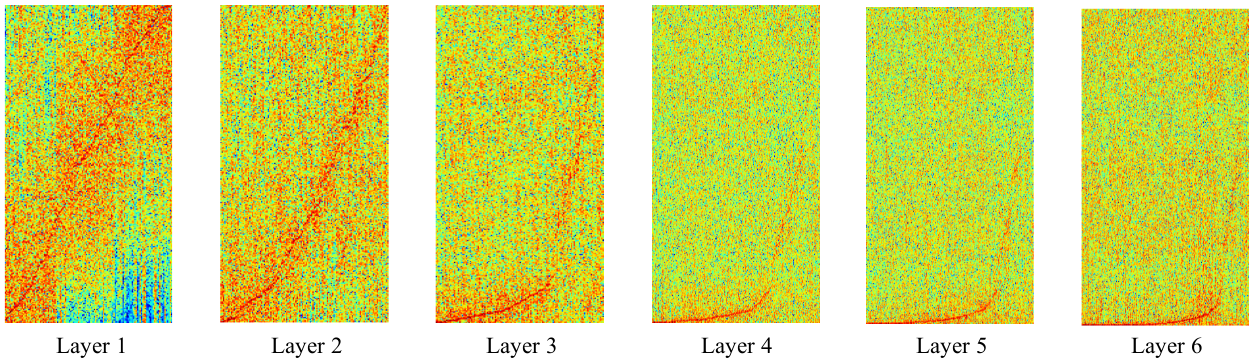
\includegraphics[scale=0.34]{wav_to_mfcc.png}
  \caption{``Spectrum of the filters in the sample-level convolution layers which are sorted by the frequency of the peak magnitude. The x-axis represents the index of the filter, and the y-axis represents the frequency'' (from \cite{wavdeep}).}
  \label{fig:wav-to-mfcc}
\end{figure}



\subsection{Models and Architectures}

Following the general trend suggested by the aforementioned comparatives (and observed in many other fields of the machine learning discipline), research based on the application of deep neural networks for end-to-end supervised learning for perceiving and predicting high-level musical features has observed a growth in quantity and success in the last years.\\

For instance, Lambert et al. combined in 2015 a network of non-linear oscilators with a deep recurrent neural network to sucessfully perceive and predict expressive rhythms\cite{expressive-rhyt}.\\

More specifially to MGR, the team of Choi et al. at the Centre for Digital Music of the Queen Mary University of London has been focusing in developing, implementing, testing and interpreting different deep learning approaches for the last few years. From their work in 2017 so far, apart from the already mentioned work reported in \cite{convtransfer} and \cite{choi-robustness}, it is worth to highlight a very interesting article in which they discuss novel techniques and approaches to interpret the process of learning and predicting high-level musical features by DCNNs\cite{choi-explaining}, especially the idea of auralisation.\\

Regarding specific architectures, they presented last year several fully-convolutional models \cite{choi-fcn}, able to learn high-level features from different domains ``such as emotion (sad, anger, happy), genre (jazz, classical) and instrumentation (guitar, strings, vocal, instrumental)'' on two different datasets, and perform multi-label tagging on them with a top performance of 0.851 AUC-ROC, which is a figure of merit that takes both precision and recall into account (see section \label{errormetrics} for more information).\\

\begin{figure}[h]
  % \hspace*{-0.6cm}
  \centering
  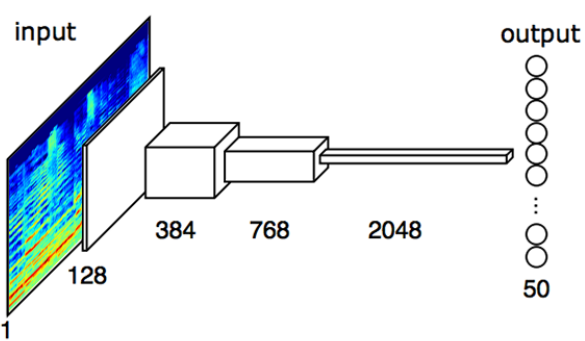
\includegraphics[scale=0.5]{fullyconv.png}
  \caption{One of the fully-convolutional neural architectures proposed in \cite{choi-fcn}. The numbers indicate the number of feature maps (i.e. channels)}
  \label{fig:wav-to-mfcc}
\end{figure}


Two months after, they presented for the same task a convolutional recurrent neural network (CRNN)\cite{choi-crnn}, which combines ``(CNNs) for local feature extraction and recurrent neural networks for temporal summarisation of the extracted features''. In the experiments they observed ``a trade-off between speed and memory: the computation of the purely convolutional network is faster than that of CRNN across all parameter settings, while the CRNN tends to outperform it with the same number of parameters''.









\section{Related Work in Carnatic R\=aga Classification} \label{context_raaga}

The task of r\=aga classification presents similar problems to the ones already exposed in section \ref{mgr-problematic} for the music genre classification: as explained by S. Gulati in 2016, ``the datasets used for evaluation by the existing methods vary immensely in terms of the number of r\=agas, the chosen set of r\=agas, the duration and the number of the audio recordings per r\=aga, and the type of audio content (monophonic or polyphonic). With such diverse datasets, it is difficult to draw any concrete conclusions on the performance of the methods across different studies. Even the survey studies such as those in Koduri et al. (2011) have not performed any exhaustive comparative evaluations on the same dataset and under the same experimental setup. Thus, creating diverse, sizable and sharable datasets that are representative of the music tradition is a potential avenue for contribution in this task. In addition to the datasets, poor description of the implementation details is another common factor amongst several existing studies. This situation becomes even more difficult as none of the approaches make their code publicly available for ensuring reproducibility of the research results''\cite[p.44]{gulati}.\\


For this reason, he opts to ``refrain from comparing the absolute r\=aga recognition accuracies across studies''\cite[p.37]{gulati}. Following this criterium, the present section will be focused on his work, since it is the most relevant for the present thesis: both this and his work are based on the same dataset, from which he is not only one of the curators (see \cite{indian-corpora}) but also its most relevant contributor to the moment. Furthermore, the dataset is ``to the best of our knowledge the largest ever used for this task''\cite[p.178]{gulati} (see chapter \ref{about-ds} for more details on the dataset).\\

Specifically, the two following sections describe ``two novel approaches for rāga recognition that jointly capture the tonal and the temporal aspects of melody'', developed by him in the context of his 2016 dissertation at the Universitat Pompeu Fabra in Barcelona. Finally, some applications of his work are also mentioned. A detailed summary of the work preceding Gulati's can be seen in Figure \ref{fig:gulati-related}.

\begin{sidewaysfigure}%[h]
  % \hspace*{-0.6cm}
  \centering
  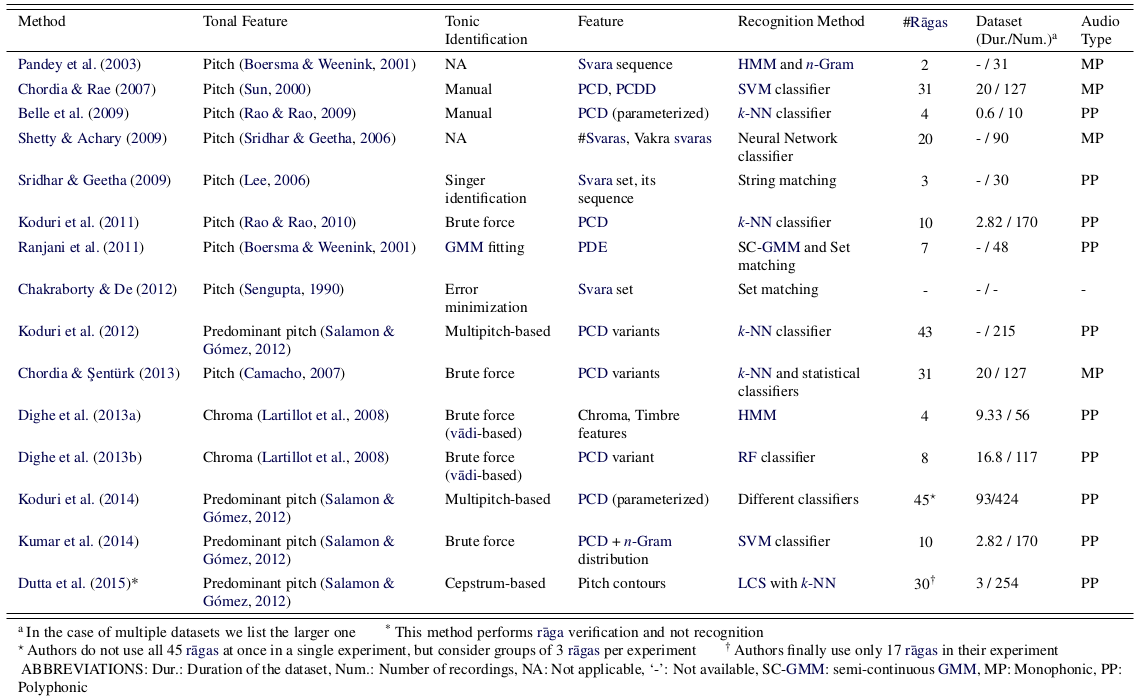
\includegraphics[scale=0.57]{gulati_related.png}
  \caption{Summary of the r\=aga recognition methods in cronological order (from \cite[p.39]{gulati})}
  \label{fig:gulati-related}
\end{sidewaysfigure}



\subsection{Vector Space Modelling (VSM) Approach}

The first approach ``employs concepts of vector space modelling to perform r\=aga recognition using melodic patterns''. It is divided in three parts: first, the audio is sent through a pipeline that is able to identify melodic patterns by extracting specific audio features. This patterns are then clustered when they are considered ``different occurrences of the same underlying melodic phrase''. Finally, and similarly to word embeddings in the text-technology field, the different clustered phrases are considered as elements of the vocabulary, and their sequence of appearance is modelled as a vector, which is finally used to detect a specific r\=aga by the type and frequency of appearance of its elements.\\

This model ``shows promising results by achieving an accuracy comparable to the state of the art method'' and ``has several advantages such as musically meaningful interpretation of the classification results''\cite[p.191]{gulati}. For instance, its experimental results ``suggest that, considering just the presence or the absence of a melodic pattern, irrespective of its frequency of occurrence, might be sufficient for r\=aga recognition. Interestingly, this finding is consistent with the fact that characteristic melodic patterns are unique to a r\=aga and a single occurrence of such patterns is sufficient to identify the r\=aga''\cite[p.186]{gulati}.\\


\subsection{Time Delayed Melodic Surface (TDMS) Approach}

This approach ``uses a novel feature, the time delayed melodic surface (TDMS). TDMS captures tonal and temporal melodic aspects that are useful in characterizing and distinguishing rāgas. TDMSs alleviate several of the shortcomings in the existing approaches and improves the accuracy of r\=aga recognition by large margins, without the use of any elaborated classification schema''. The only drawback for that is that it ``seeks to abstract the melody representation'', giving up some of its interpretability.\\

As explained in\cite[p.192]{gulati}, the computation of a TDMS involves three steps: pre-processing (which normalizes a low-level representation of the melody with respect to the tonic pitch), surface generation (a two-dimensional discretized histogram of the elements of the pre-processed melody), and post-processing (consisting on applying some compression and smoothing to the surface). Figure \ref{fig:tdms} shows an example of such surface, before and after post-processing.\\

All the proposed variants of this method scored at least 81.5\% of accuracy when applied to the 40 r\=agas of the \(RRD_{CMD}\) dataset (described in chapter \ref{about-car}).


\begin{figure}[h]
  \centering
  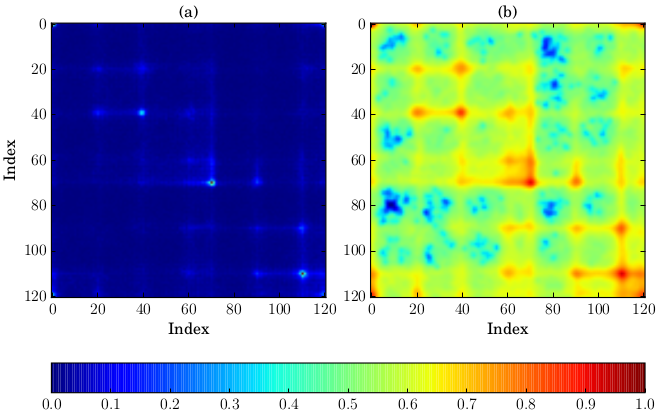
\includegraphics[scale=0.5]{tdms.png}
  \caption{An example of the generated TDMS for a music piece in r\=aga Yaman, before (a) and after (b) applying post-processing (from \cite[p.195]{gulati})}
  \label{fig:tdms}
\end{figure}


\subsection{Applications}

The results of Gulati's work have already found several applications. One of them is the {\it raagawise}\cite{raagawise} web-application, which performs r\=aga recognition based on an incoming audio stream. Another remarkable one is the tonic identification software present in the Dunya platform (described in section \ref{compmsc}). Figure \ref{fig:dunya-player} shows a screenshot of the platform's audio player, wich besides the raw audio wave displays its extracted melodic and spectral features.

\begin{figure}[h]
  \centering
  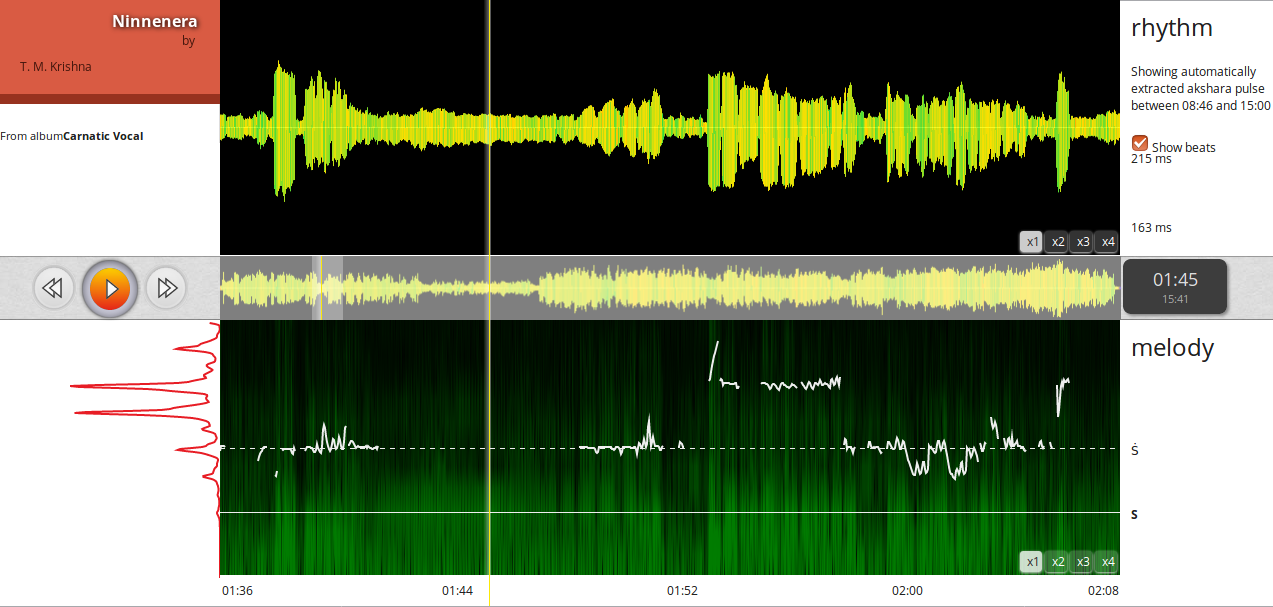
\includegraphics[scale=0.33]{dunya_player.png}
  \caption{A screenshot of the main section of Dunya's music player. Note the extracted melodic and spectral features.}
  \label{fig:dunya-player}
\end{figure}
